\documentclass[12pt]{article}
\usepackage[T1]{fontenc}
\usepackage[utf8]{inputenc}
\usepackage{sbc-template}
\usepackage{graphicx}
\usepackage[hyphens]{url}
\usepackage{float}
\usepackage[brazilian]{babel}
\usepackage{microtype}
\usepackage{lmodern}
\makeatletter
\g@addto@macro{\UrlBreaks}{%
  \do\/\do\-\do\.\do\:\do\a\do\b\do\c\do\d\do\e\do\f\do\g\do\h\do\i\do\j\do\k\do\l\do\m\do\n\do\o\do\p\do\q\do\r\do\s\do\t\do\u\do\v\do\w\do\x\do\y\do\z % chktex 4
  \do\A\do\B\do\C\do\D\do\E\do\F\do\G\do\H\do\I\do\J\do\K\do\L\do\M\do\N\do\O\do\P\do\Q\do\R\do\S\do\T\do\U\do\V\do\W\do\X\do\Y\do\Z%
  \do\0\do\1\do\2\do\3\do\4\do\5\do\6\do\7\do\8\do\9%
} % chktex 4
\makeatother

\sloppy

\title{Avaliação de Desempenho de Bibliotecas de Processamento de Dados\\ em Ambiente com Recursos Limitados}

\author{Denilson Silva Lima\inst{1}, Emerson Neves dos Santos\inst{1}, \\
  Felipe Andrade dos Santos Carvalho\inst{1}, \\
  Maiko André Antunes de Sousa\inst{1}}

\address{Tecnologia em Análise e Desenvolvimento de Sistemas\\
  Instituto Federal de Educação, Ciência e Tecnologia Baiano\\ Campus Guanambi\\
  Guanambi-BA, Brasil
  \email{\{denisilvalima536.com, emersonnevess80,}
  \email{felipebaiano04, maikosousa.tech\}}
  \email{@gmail.com}
}

\makeatletter
\def\@cite#1#2{({#1\if@tempswa, #2\fi})}
\makeatother

\begin{document} 

\maketitle

\begin{resumo} 
  Este estudo apresenta um benchmark comparativo de desempenho entre as bibliotecas Pandas, Polars, DuckDB e PySpark em ambiente com recursos de hardware limitados. A avaliação utilizou um planejamento fatorial com três tamanhos de datasets (256MB, 512MB e 1GB) e quatro operações analíticas (filtragem, agregação, junção e ordenação). Para garantir a estabilidade das medições, cada teste foi executado de forma estanque por subprocessos individuais, precedidos por warmup. Os resultados experimentais sugerem que o Pandas apresenta maior demanda de RAM em grandes volumes, o Polars e o DuckDB indicam maior eficiência temporal e de memória, enquanto o PySpark sugere maior overhead de inicialização local.
\end{resumo} 

\begin{abstract}
  This study presents a comparative performance benchmark among Pandas, Polars, DuckDB, and PySpark in hardware-constrained environments. The evaluation employed a full factorial design with three dataset sizes (256MB, 512MB, and 1GB) and four analytical operations (filtering, aggregation, joining, and sorting). To ensure measurement stability, each test was executed independently using individual subprocesses preceded by warmup. The experimental results suggest that Pandas demands more RAM at larger volumes, Polars and DuckDB show signs of higher time and memory efficiency, while PySpark suggests higher local initialization overhead.
\end{abstract}
     
\newpage

\section{Introdução}

O processamento de dados desempenha papel essencial em áreas como ciência de dados, engenharia de
dados e análise computacional, envolvendo operações como limpeza, transformação, filtragem e
agregação de informações~\cite{moutinho:2024}. Com o crescimento do volume de dados e da
complexidade das aplicações, as bibliotecas de processamento passaram a exercer influência direta no
desempenho, no consumo de memória e na escalabilidade das soluções
computacionais~\cite{cirillo:2025}.

Nesse contexto, os benchmarks tornam-se importantes para avaliar experimentalmente diferentes
ferramentas em cenários semelhantes de execução, permitindo analisar métricas como tempo de
processamento, utilização de recursos e eficiência operacional~\cite{cirillo:2025}. Além disso,
diferentes bibliotecas adotam abordagens arquiteturais distintas, priorizando aspectos como
simplicidade de uso, paralelismo, processamento otimizado ou escalabilidade distribuída. Assim, a
comparação entre ferramentas como Pandas, Polars, DuckDB e PySpark possibilita compreender os
principais trade-offs relacionados ao desempenho e ao consumo de recursos em diferentes cenários de
uso.

\subsection{Processamento de Dados em Ambientes com Recursos Limitados}

Ambientes computacionais com recursos limitados de hardware, como restrições de memória RAM, CPU e
armazenamento, impõem desafios severos ao processamento de volumes crescentes de dados, tornando a
eficiência das bibliotecas um fator crucial para evitar falhas operacionais e garantir o desempenho
adequado~\cite{ourique:2024}. Diante desse cenário, avaliar o gerenciamento de memória, o
paralelismo e a escalabilidade das ferramentas sob restrições permite identificar aquelas que
apresentam o melhor equilíbrio entre velocidade de execução e consumo de
recursos~\cite{cirillo:2025}. Assim, estudos comparativos são fundamentais para orientar a escolha
da solução mais adequada de acordo com o contexto de hardware disponível e o volume de dados a ser
manipulado~\cite{cirillo:2025}.


\subsection{Objetivos e Contribuições deste Estudo}

Este estudo experimental contribui para orientar desenvolvedores e engenheiros de dados ao avaliar
sistematicamente quatro abordagens arquiteturais distintas de manipulação de dados em Python:
Pandas, Polars, DuckDB e PySpark. As principais contribuições deste trabalho consistem em:

\begin{itemize}
    \item Avaliação fatorial completa em ambiente com isolamento estrito por subprocessos sob limitação real de hardware.
    \item Quantificação direta e comparativa do pico de consumo de memória física e tempo de execução analítico em três volumes de escala (256MB, 512MB e 1GB).
    \item Identificação clara dos trade-offs de desempenho e confiabilidade operacional.
\end{itemize}

\section{Bibliotecas de Processamento de Dados}

Esta seção apresenta uma visão geral das quatro bibliotecas avaliadas neste estudo, destacando seus
objetivos de design, características arquiteturais e mecanismos para lidar com restrições de
hardware.

\subsection{Pandas}

O Pandas é uma das principais bibliotecas de código aberto para manipulação e análise de dados
estruturados em Python, amplamente reconhecida pela simplicidade de suas estruturas de
\textit{Series} e \textit{DataFrame} e suporte a diversos formatos de arquivos~\cite{mckinney:2012,
pandas:docs}.

Apesar de sua popularidade e maturidade, a biblioteca apresenta limitações significativas em
cenários com grandes volumes de dados ou recursos computacionais restritos, decorrentes de seu
modelo de processamento majoritariamente em memória (\textit{in-memory}) e sem paralelismo
nativo~\cite{pandas:docs}. Ainda assim, sua estabilidade e ampla compatibilidade com o ecossistema
Python a consolidam como uma referência indispensável para estudos comparativos de desempenho.


\subsection{Polars}

O Polars é uma biblioteca de processamento de dados desenvolvida em Rust para manipulação eficiente
de tabelas, utilizando o formato colunar do Apache Arrow para otimizar o uso de memória e
cache~\cite{polars:2026}. Diferenciando-se do Pandas, foi projetado com foco em alto desempenho,
oferecendo processamento paralelo nativo, execução vetorizada, avaliação preguiçosa (\textit{lazy
evaluation}) para otimização de consultas e suporte a processamento fora da memória (\textit{out-of-
core})~\cite{nvidia:2026, polars:2026}. Essas características minimizam o tempo de execução e a
pegada de recursos computacionais, tornando o Polars ideal para cenários com grandes volumes de
dados ou hardware restrito.


\subsection{DuckDB}

O DuckDB é um sistema de gerenciamento de banco de dados analítico (OLAP) embarcado e de código
aberto (\textit{in-process}). Ele é associado frequentemente ao conceito de ``SQLite para análises''
devido à sua simplicidade de uso e ao alto desempenho em consultas analíticas~\cite{duckdb:2026a,
duckdb:2026b}.

A ferramenta emprega armazenamento colunar, execução vetorizada e suporte nativo a formatos como
CSV, Parquet e Apache Arrow, proporcionando alta eficiência em operações analíticas como agregações,
filtros e junções~\cite{duckdb:ai2026}. Um de seus principais diferenciais em relação a soluções
puramente em memória é a capacidade de processar volumes de dados maiores que a RAM disponível por
meio de mecanismos de descarregamento em disco (\textit{spill to disk}). Isso o torna altamente
relevante para cenários com recursos computacionais limitados~\cite{duckdb:2026a}.


\subsection{Apache Spark (PySpark)}

O PySpark é a interface em Python do Apache Spark, uma plataforma de código aberto voltada ao
processamento de dados distribuídos em larga escala (\textit{Big Data}) por meio de RDDs e
DataFrames otimizados pelo mecanismo Catalyst. Ao contrário das demais ferramentas avaliadas, ele
opera sobre a Máquina Virtual Java (JVM) e utiliza a arquitetura distribuída mestre-trabalhador
(Driver-Executor) projetada para clusters.
\newpage
Embora ofereça alta escalabilidade e tolerância a falhas, seu modelo de execução acarreta um elevado
consumo basal de RAM e CPU decorrente da inicialização da JVM e da serialização de dados entre
processos Python e Java\@. Essa característica torna essencial sua avaliação neste estudo para
determinar os limites práticos e a viabilidade da plataforma em ambientes de nó único e recursos
severamente limitados.


\section{Desenvolvimento da Análise}

Para realizar a medição e análise de desempenho entre as referidas bibliotecas de processamento de
dados, foi desenvolvido um programa computacional escrito na linguagem Python, que executa nas
quatro bibliotecas as operações de: filtragem, junção, agregação e ordenação. Em paralelo, o
programa realiza a medição do consumo de recursos computacionais requisitados por cada biblioteca, a
fim de gerar um arquivo JSON com os resultados de desempenho obtidos. A partir do arquivo gerado,
inicia-se a análise estatística do benchmark.

O programa desenvolvido executa os seguintes passos: (1) prepara os dados de entrada de acordo com
os tamanhos definidos para o teste; (2) itera pelas bibliotecas selecionadas; (3) para cada
biblioteca, executa e afere o tempo e o consumo de memória máxima |na fase de carregamento do
dataset; (4) executa iterações consecutivas das operações analíticas (filtragem, junção, ordenação e
agregação) sob um isolamento estrito de subprocessos, registrando os picos de desempenho; e (5)
salva e consolida estruturadamente todos os dados coletados em formato JSON\@.

\subsection{Conjunto de Dados Utilizado}

Os experimentos foram conduzidos utilizando dados agrupados do Sistema Único de Saúde (SUS), referentes aos casos de Dengue registrados no Brasil no ano de 2024. Esse conjunto de dados foi obtido publicamente a partir da plataforma Kaggle, por meio do repositório \url{https://www.kaggle.com/datasets/henriquerezermosqur/dados-sus-sinan-dengue-2021-2024}, servindo como base realista para a avaliação de desempenho e de escalabilidade das bibliotecas sob teste. A partir dessa base original, os três datasets (256MB, 512MB e 1GB) foram gerados estimando-se a quantidade média de bytes por linha e realizando a subamostragem ou duplicação cíclica e concatenação de registros até que a volumetria desejada fosse alcançada com precisão. % chktex 8

\subsection{Ambiente de Execução}


Neste experimento, o ambiente de execução escolhido foi um notebook Dell Inspiron \mbox{15-3583}, % chktex 8
com as seguintes especificações: Processador Intel de 8ª geração (\mbox{i7-8565U}), 8GB de memória % chktex 8
RAM DDR4 a 2400 MHz distribuídos em um slot SODIMM, SSD NVMe de 256GB M.2 PCIe, placa integrada
Intel UHD Graphics 620 e sistema operacional Arch Linux versão minimal (sem interface gráfica). Ao iniciar o sistema sem carregar a interface gráfica, apenas os processos essenciais relacionados ao kernel e ao terminal permanecem em execução, minimizando o ruído computacional de fundo. Esse
hardware foi escolhido por representar um ambiente limitado para análise de dados, onde cada recurso
é indispensável para possibilitar a execução das bibliotecas selecionadas de forma controlada.

\subsection{Definição da Variável de Resposta, Fatores e Níveis}

Para essa análise comparativa entre as bibliotecas de processamento de dados escolhidas, foram
selecionadas duas variáveis de respostas: o tempo de execução (medido em segundos) e o consumo de
memória (medido em Megabytes). Essas variáveis foram selecionadas por indicar métricas diretamente
ligadas à limitação de hardware em dispositivos modestos, possibilitando assim uma comparação
realista entre as referidas bibliotecas.

O comportamento dessas variáveis de resposta foi definido em função de três fatores de controle
independentes, cada um com seus respectivos níveis:
\begin{itemize}
    \item \textbf{Biblioteca selecionada:} contendo quatro níveis: Pandas, Polars, DuckDB e PySpark.
    \item \textbf{Tamanho do dataset:} submetido ao processamento, contendo três níveis: 256MB, 512MB e \mbox{1GB}\@.
    \item \textbf{Operação analítica:} executada sobre os dados, dividida em quatro níveis: filtragem, agregação, junção e ordenação.
\end{itemize}
\subsection{Execuções}

O experimento adota o método de planejamento fatorial completo, abrangendo todas as combinações
possíveis entre as quatro bibliotecas, os três tamanhos de dataset e as quatro operações analíticas,
resultando em um arranjo de 48 cenários experimentais executados ao longo de 48 iterações
consecutivas, totalizando 2.304 execuções. Para assegurar uma comparação justa e fiel da eficiência computacional, o critério de
parada foi definido estritamente pela quantidade total de registros processados, garantindo que
todas as ferramentas executem exatamente a mesma carga de trabalho em cada teste.

Para mitigar o impacto de vazamentos de memória (\textit{memory leaks}) ou acúmulo de cache, cada
execução individual é isolada em um novo subprocesso do sistema operacional, permitindo registrar
falhas de falta de memória (OOM) de forma segura sem interromper a estabilidade da suíte de testes.
Adicionalmente, o fluxo experimental é dividido nas fases de carregamento (\textit{load}) e de
operação — que inclui uma iteração preliminar de aquecimento (\textit{warmup}) para desconsiderar
atrasos de inicialização de módulos e compilações JIT —, consolidando todos os tempos de execução e
picos de uso de memória física (RAM) em um arquivo JSON para posterior análise estatística.

\newpage
\section{Resultados obtidos}

Esta seção apresenta os resultados experimentais obtidos a partir da execução do benchmark
projetado. As análises estão estruturadas em três vertentes principais: a escalabilidade temporal
das operações analíticas, a eficiência no consumo de memória RAM (com ênfase no limite físico de
hardware de 8GB) e a estabilidade das ferramentas ao longo de rodadas repetidas de teste.


\subsection{Curva de Escalabilidade Temporal}
\begin{figure}[H]
\centering

\includegraphics[width=0.8\textwidth]{assets/escalabilidade_tempo.pdf}
\caption{Curva de Escalabilidade (Tempo de Execução em escala log) por Operação nas Diferentes Bibliotecas.}\label{fig:escalabilidade}
\end{figure}

O desempenho de processamento de cada biblioteca foi avaliado para as quatro operações analíticas
principais (filtragem, agregação, junção e ordenação) em função do aumento volumétrico dos dados
(256MB, 512MB e 1GB). Os tempos médios das 48 rodadas estão expressos no gráfico de escalabilidade
na Figura~\ref{fig:escalabilidade}.

Observa-se que o PySpark exibe, sistematicamente, o maior tempo de processamento em todas as
operações analíticas, situando-se entre $10^0$ e $2\cdot 10^1$ segundos. Esse comportamento reflete
o custo computacional severo decorrente da inicialização de sua infraestrutura local (JVM, drivers e
workers), além da necessária serialização de objetos entre os ambientes Python e Java. Em
contrapartida, o Polars e o DuckDB mostram-se extremamente eficientes, mantendo tempos de execução
subsegundo (frequentemente na escala de milissegundos, $10^{-2}$ s). % chktex 13

Na operação de filtragem, o Pandas apresenta excelente desempenho para volumes baixos (256MB), sendo
ligeiramente mais rápido que o Polars e o DuckDB\@. Contudo, em operações mais complexas e pesadas
como a junção (\textit{join}), o Pandas demonstra baixa escalabilidade temporal: enquanto o Pandas
requer cerca de $0,8$ s para o processamento de 1GB, o Polars e o DuckDB executam a mesma carga em
apenas $0,01$ s, operando em uma velocidade aproximadamente 80 vezes superior.

\newpage
\subsection{Eficiência no Consumo de Memória RAM}

Considerando que o ambiente computacional avaliado possui restrição física de hardware, a eficiência
de alocação de memória é um fator crítico de confiabilidade operacional. A Figura~\ref{fig:ram}
ilustra o consumo de pico de memória (RSS) das ferramentas para cada operação durante o
processamento de 1GB\@.

\begin{figure}[!ht]
\centering
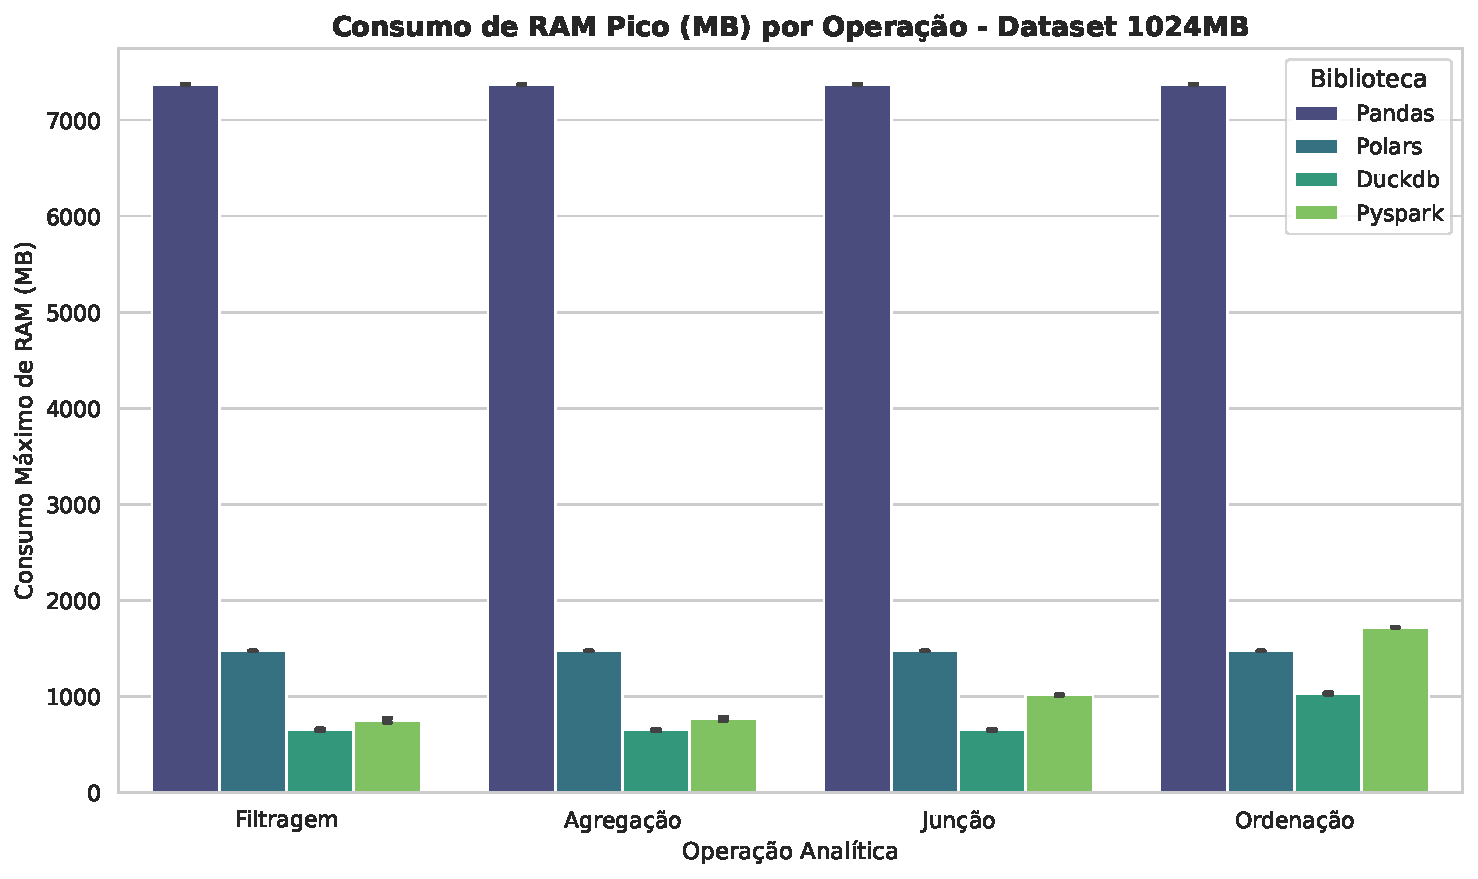
\includegraphics[width=0.8\textwidth]{assets/consumo_ram_1gb.pdf}
\caption{Pico de Consumo de RAM (MB) por Operação no Dataset de 1024MB.}\label{fig:ram}
\end{figure}

Os resultados evidenciam que o Pandas aloca constantemente em torno de 7.400 MB de RAM para executar
qualquer transformação em 1GB de dados. Essa alocação estática e em memória física consome quase
93\% da capacidade total de hardware disponível, colocando o sistema no limiar de falhas de falta de
memória (Out-Of-Memory, ou OOM) em ambientes produtivos limitados.

Por outro lado, o DuckDB destaca-se como a ferramenta mais econômica, operando de forma constante na
faixa de 600 a 650 MB\@. Isso é possibilitado por sua arquitetura analítica embarcada que emprega
descarregamento dinâmico em disco (\textit{spill-to-disk}) e processamento vetorizado por blocos. O
Polars consolidou-se em uma posição intermediária eficiente, estabilizando seu pico de consumo em
torno de 1.500 MB, enquanto o PySpark flutuou entre 700 MB e 1.700 MB\@.

Para fins de análise comparativa com volumes menores, as Figuras~\ref{fig:ram_512} e~\ref{fig:ram_256} ilustram o consumo de pico de memória RAM para os conjuntos de dados de 512MB e 256MB, respectivamente.

\begin{figure}[!ht]
\centering
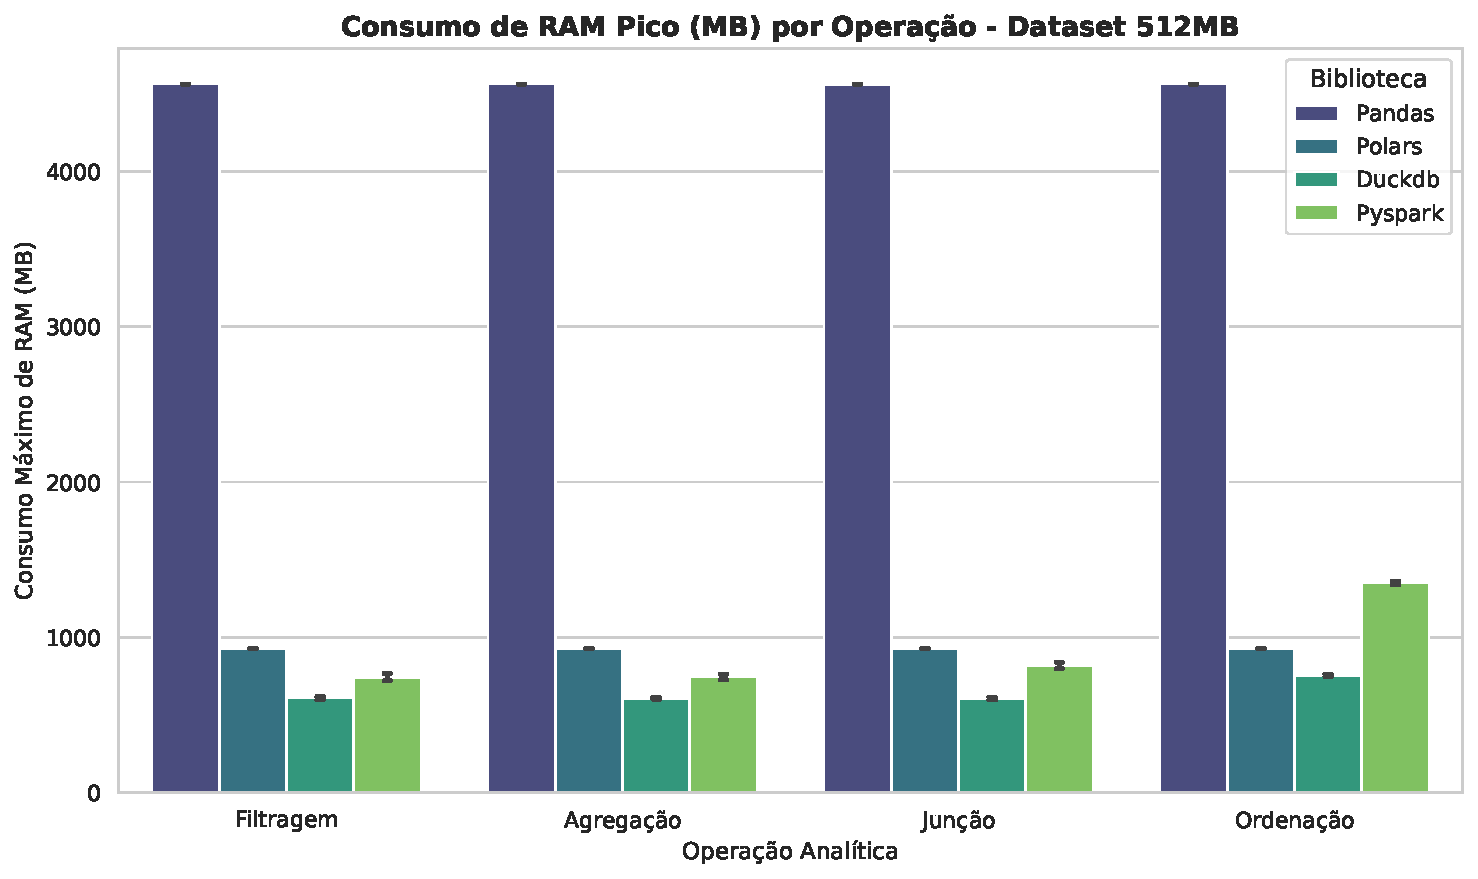
\includegraphics[width=0.8\textwidth]{assets/consumo_ram_512mb.pdf}
\caption{Pico de Consumo de RAM (MB) por Operação no Dataset de 512MB.}\label{fig:ram_512}
\end{figure}

\newpage
Ao duplicar o volume para 512MB (Figura~\ref{fig:ram_512}), o consumo do Pandas escala proporcionalmente, atingindo aproximadamente 4.560 MB de alocação de RAM, o que representa cerca de 57\% da capacidade total de hardware. O Polars eleva seu patamar de consumo para aproximadamente 928 MB\@. O DuckDB permanece como a solução mais eficiente em termos de memória, operando em cerca de 605 a 610 MB para as operações de filtragem, agregação e junção, e atingindo 755 MB na ordenação. O PySpark, por sua vez, mantém-se estável nas operações de filtragem e agregação (cerca de 744 MB), mas cresce para 817 MB na junção e 1.350 MB na ordenação. Esses comportamentos confirmam a tendência de crescimento linear do consumo de memória para o Pandas e o Polars, enquanto DuckDB e PySpark mostram uma curva mais amortecida devido ao gerenciamento dinâmico e custo fixo de suas respectivas infraestruturas.

\begin{figure}[!ht]
\centering
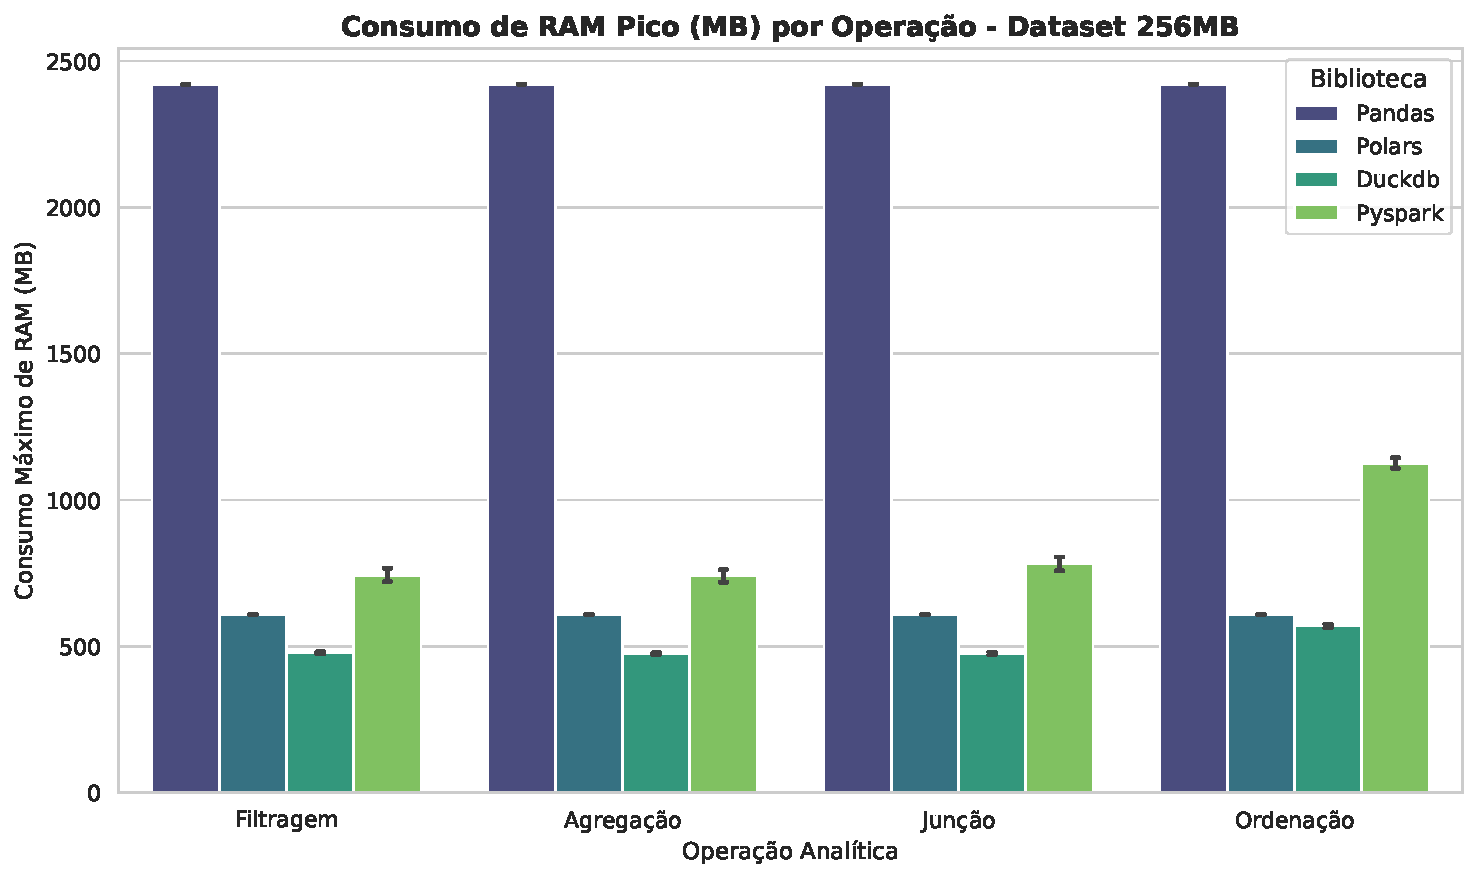
\includegraphics[width=0.8\textwidth]{assets/consumo_ram_256mb.pdf}
\caption{Pico de Consumo de RAM (MB) por Operação no Dataset de 256MB.}\label{fig:ram_256}
\end{figure}
No cenário de 256MB (Figura~\ref{fig:ram_256}), o Pandas apresenta um pico de consumo estável em torno de 2.420 MB para todas as operações, o que equivale a cerca de 9,4 vezes o volume nominal dos dados de entrada. O Polars e o DuckDB mantêm perfis de consumo otimizados: o Polars estabiliza-se em aproximadamente 609 MB, enquanto o DuckDB demanda em média 475 MB para filtragem, agregação e junção, com uma elevação para cerca de 569 MB na operação de ordenação. O PySpark exibe um consumo médio de 740 MB nas operações de filtragem e agregação, elevando-se a 783 MB na junção e alcançando 1.125 MB na ordenação, evidenciando o impacto da JVM mesmo em volumes menores.

\subsection{Estabilidade e Dispersão de Desempenho}

Para avaliar a consistência das ferramentas frente a flutuações e eventuais custos de aquecimento de
compilação JIT ou Garbage Collection, a distribuição estatística das execuções no dataset de 1GB é
sumarizada na Figura~\ref{fig:estabilidade}.

\begin{figure}[!ht]
\centering
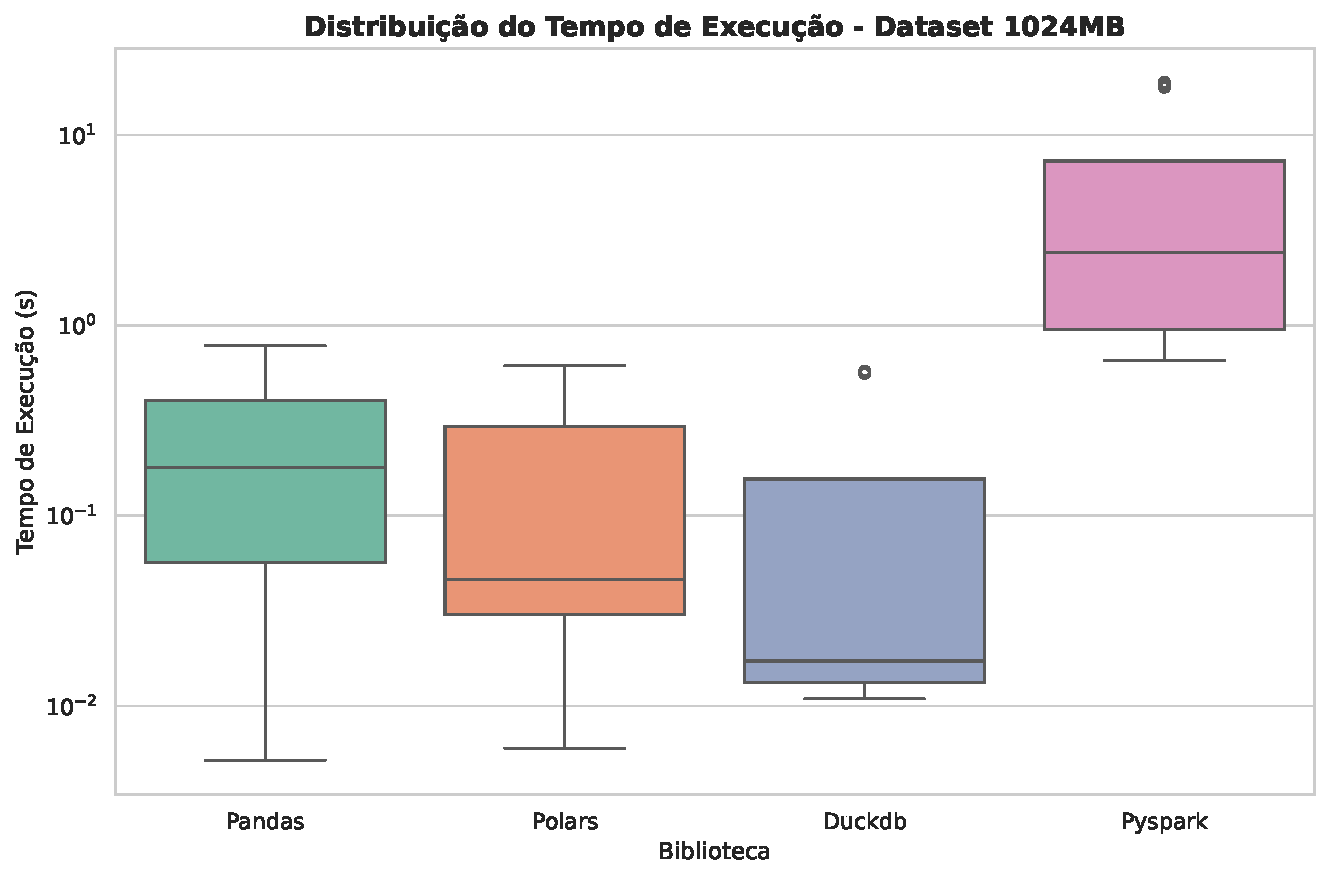
\includegraphics[width=0.7\textwidth]{assets/estabilidade_tempo.pdf}
\caption{Boxplot de Distribuição do Tempo de Execução no Dataset de 1024MB.}\label{fig:estabilidade}
\end{figure}

O DuckDB obteve a menor mediana de tempo geral, apresentando apenas um \textit{outlier} superior
(cerca de 0,6 s) referente à primeira iteração analítica. O Polars apresentou a maior consistência
de estabilidade geral, exibindo uma dispersão extremamente compacta e sem quaisquer
\textit{outliers}. O PySpark, por sua vez, demonstrou alta volatilidade e dispersão, com tempos
oscilando entre 0,6 s e 7 s, além de registrar um pico atípico próximo a 20 segundos, o que reflete
a instabilidade do Garbage Collection da JVM sob restrição severa de recursos.

\newpage
\section{Considerações Finais}

Este trabalho apresentou uma análise comparativa experimental preliminar entre Pandas, Polars, DuckDB e PySpark em um cenário específico de hardware restrito.

Os resultados obtidos indicam que a escolha da biblioteca de processamento de dados pode influenciar a eficiência e a estabilidade do sistema sob restrição de recursos. A partir do caso de teste analisado, o Pandas demonstrou tendências de maior consumo de memória RAM, indicando que seu uso poderia ser menos adequado para volumes de dados que se aproximam do limite físico da máquina. O PySpark, embora projetado para processamento distribuído, apresentou maior overhead temporal quando executado localmente em um único nó.

Por outro lado, o Polars e o DuckDB apontaram indícios de serem alternativas eficientes para cenários de hardware limitado, apresentando um comportamento otimizado na alocação de memória e no tempo de execução sob as condições deste experimento. Contudo, as observações deste trabalho limitam-se ao escopo experimental avaliado, não permitindo generalizações definitivas. Como trabalhos futuros, sugere-se a ampliação deste benchmark para outros formatos de dados e a realização de testes com volumes significativamente maiores, a fim de corroborar ou aprofundar as tendências observadas.

\bibliographystyle{sbc} \bibliography{sbc-template}

\end{document}

